\documentclass[a4paper]{article}
\usepackage[utf8]{inputenc}
\usepackage[russian,english]{babel}
\usepackage[T2A]{fontenc}
\usepackage[left=10mm, top=20mm, right=18mm, bottom=15mm, footskip=10mm]{geometry}
\usepackage{indentfirst}
\usepackage{amsmath,amssymb}
\usepackage[italicdiff]{physics}
\usepackage{graphicx}
\usepackage{multirow}
\usepackage{svg}
\graphicspath{{images/}}
\DeclareGraphicsExtensions{.pdf,.png,.jpg}
\usepackage{wrapfig}
\usepackage{caption}
\captionsetup[figure]{name=Рисунок}
\captionsetup[table]{name=Таблица}
\title{\underline{Определение теплоты испарения жидкости}}
\author{Каспаров Николай, Б01-304}

\begin{document}

\maketitle
\begin{center}
\Large{\textbf{ }}
\end{center}

\subparagraph{Цель работы:}
Вычисление теплоты испарения воды.

\subparagraph{В работе используются}
Термостат, подключенный к герметичному сосуду с водой; термометр; ртутный манометр;
отсчетный микроскоп, штангентциркуль

\section{Теоретическое введение}

Как известно, при испарении с поверхности жидкости вылетают молекулы,
обладающие достаточной кинетической энергией, что приводит к тому, что
жидкость теряет быстрые молекулы и охлаждается.
Поэтому чтобы точно измерить теплоты испарения, придется подводить к воде тепло.
Однако такой метод не позволяет получить точные результаты из-за неконтролируемых
потерь тепла.

В данной работе используется другой метод, основанный на формуле Клапейрона-Клаузиуса:

\begin{equation}
    \frac{dP}{dT} = \frac{L}{T(V_2 - V_1)}
\end{equation}

Пренебрегая $V_1$ и используя уравнение идеального газа получим:

\begin{equation}
    L = \frac{RT^2}{P} \frac{dP}{dT} = -R \frac{d(\ln{P})}{d(1/T)}
\end{equation}

\section{Экспериментальная установка}

\begin{figure}[h!]
    \centering
    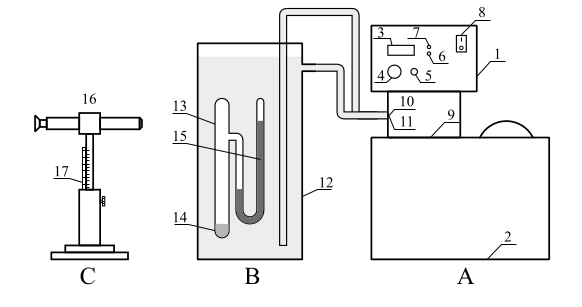
\includegraphics[scale=0.6]{stand.png}
\end{figure}

Эспериментальная установка состаит из (12) емкости с водой,
подключенной (А) термостату, способному поддерживать постоянную заданную температуру воды.
В емкость (12) погружен запаянный прибор (13) с водой (14).
Давление воды опреденяется ртутным манометром (15). Численная величина давления
измеряется по разности показаний, полученных с помощью микроскопа (16), 
подключенного к штангентцирклю (17).

\newpage

\section{Выполнение}
\subsection{Экспериментальные данные}

\begin{figure}[h!]
    \centering
    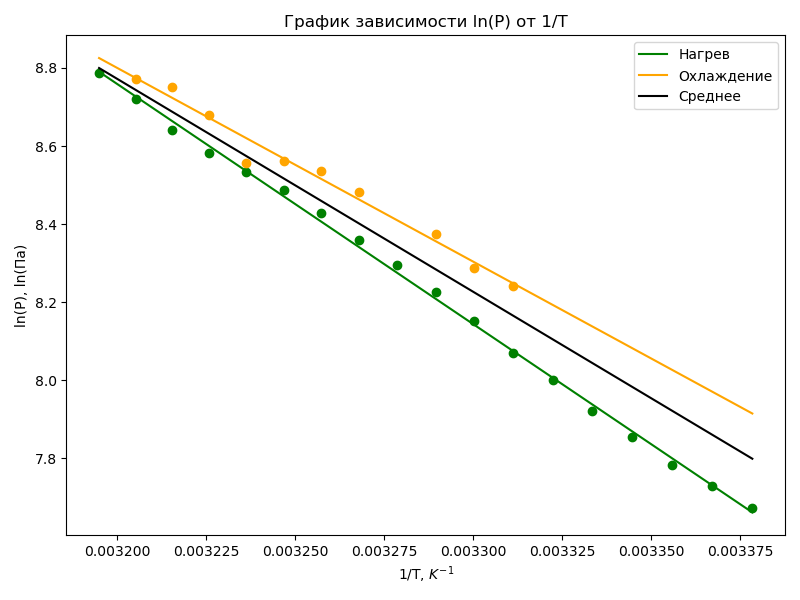
\includegraphics[scale=0.85]{figure1.png}
\end{figure}

Как мы можем видеть, значения при нагревании плохо совпадают с аналогичными
при нагревании:


\begin{equation}
    L_\text{нагр} = (2840 \pm 30) \ \text{мДж / кг}
\end{equation}
\begin{equation}
    L_\text{охл} = (2300 \pm 120) \ \text{мДж / кг}
\end{equation}
\begin{equation}
    L_\text{сред} = (2500 \pm 150) \ \text{мДж / кг}
\end{equation}

Выберем среднее значение, так как оно учитывает в себе ошибку, заключенную
в недостаточном ожидании достижения равновесного состояния жидкости в термостате
с исследуемой.

Сравним с табличным значением:

\begin{equation}
    L_\text{табл} = 2437 \ \text{мДж / кг}
\end{equation}

Мы попали в пределах погрешности!

\newpage

Теперь построим график давления насыщенных паров от температуры

\begin{figure}[h!]
    \centering
    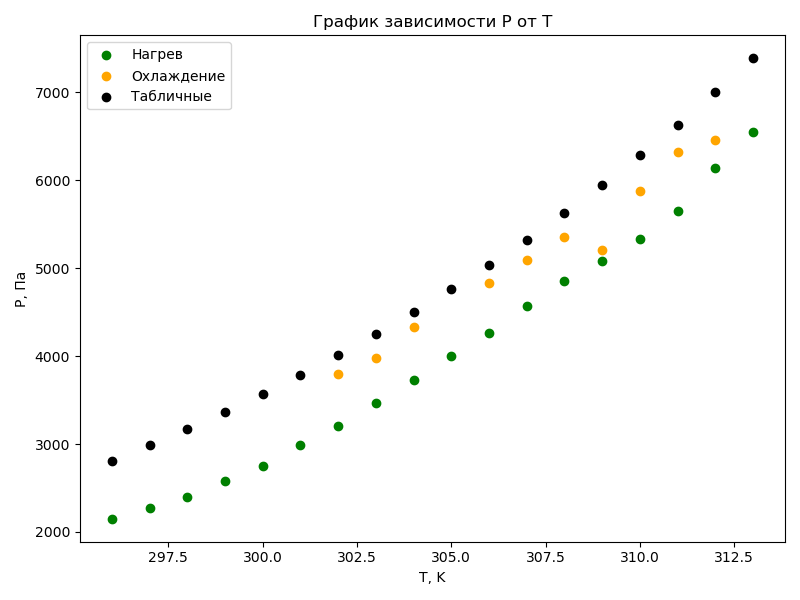
\includegraphics[scale=0.85]{figure2.png}
\end{figure}

Как мы можем видеть, из-за недостаточной рефлексации системы, значения лишь
приближаются к реальным

\section{Итоги}

Используя установку, мы сняли 18 показаний при нагревании и 10 при охлаждении
с 23 до 40 градусов.

Используя общий график $ln(P)(1/T)$ мы смогли попасть в табличные значения теплоты 
испарения воды с учетом погрешности.
\begin{equation*}
    L_\text{получ} = (2500 \pm 150) \ \text{мДж / кг}
\end{equation*}
\begin{equation*}
    L_\text{табл} = 2437 \ \text{мДж / кг}
\end{equation*}
Однако по-отдельности данные при нагревании и охлаждении показали неверные результаты.

Это обусловлено недостаточным временем релаксации, о чем говорит
разница между значениями при нагревании и охлаждении.

Также график зависимости P(T) довольно точно описывает значения 
давления насыщенных паров от температуры при охлаждении, чего нельзя сказать
про нагревание (что было бы сложно предсказать, не используя значения из таблицы).
Аналогично, проблема возникает из-за низких времен релаксации.

\end{document}
